\subsection{Realizar backup en Windows con Bacula}

\textbf{Configuración de Filesets}

Primero, vamos a la sección de Filesets en la interfaz de Webmin de Bacula.

\begin{figure}[H]
    \centering
    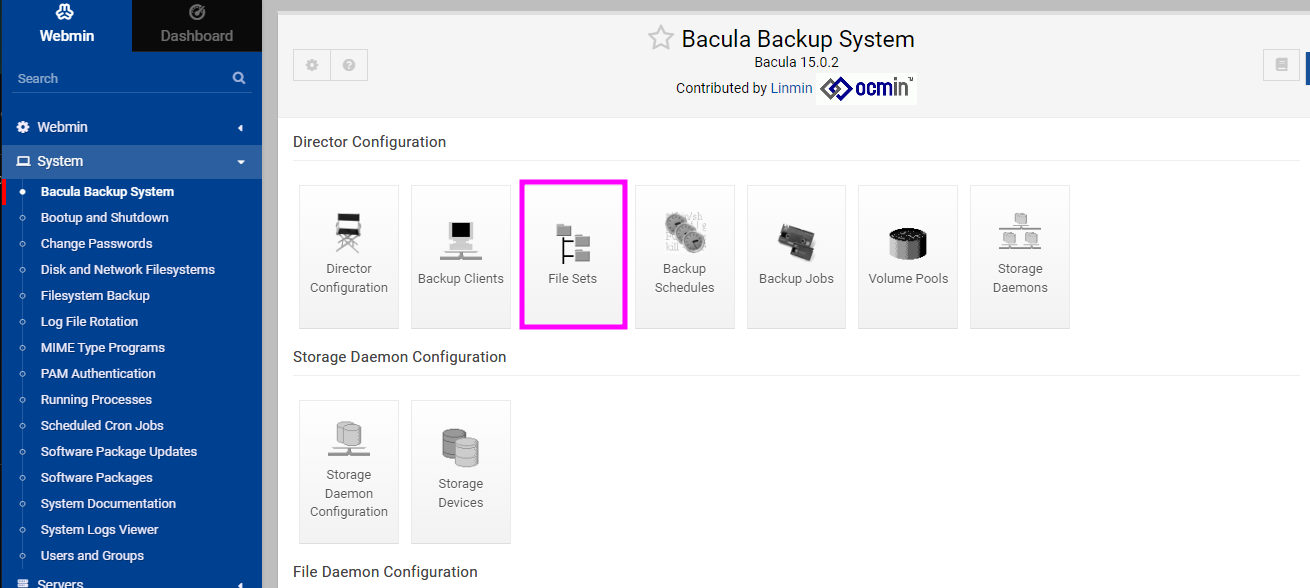
\includegraphics[width=0.5\linewidth]{instalacionBacula/filesetwebmin.png}
    \caption{Acceso a Filesets en Webmin.}
\end{figure}

Creamos un nuevo Fileset para especificar qué archivos queremos respaldar. Este será específico para Windows, incluyendo documentos importantes.

\begin{figure}[H]
    \centering
    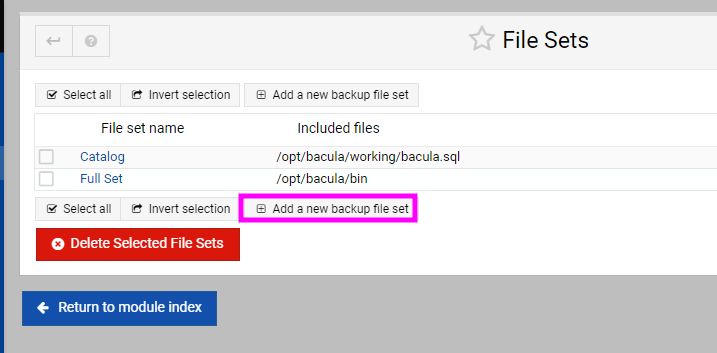
\includegraphics[width=0.5\linewidth]{instalacionBacula/cpropiofileset.png}
    \caption{Creación de un nuevo Fileset.}
\end{figure}

Definimos las opciones necesarias para el Fileset, como los directorios a respaldar, el tipo de firma de archivos, y las opciones de compresión.

\begin{figure}[H]
    \centering
    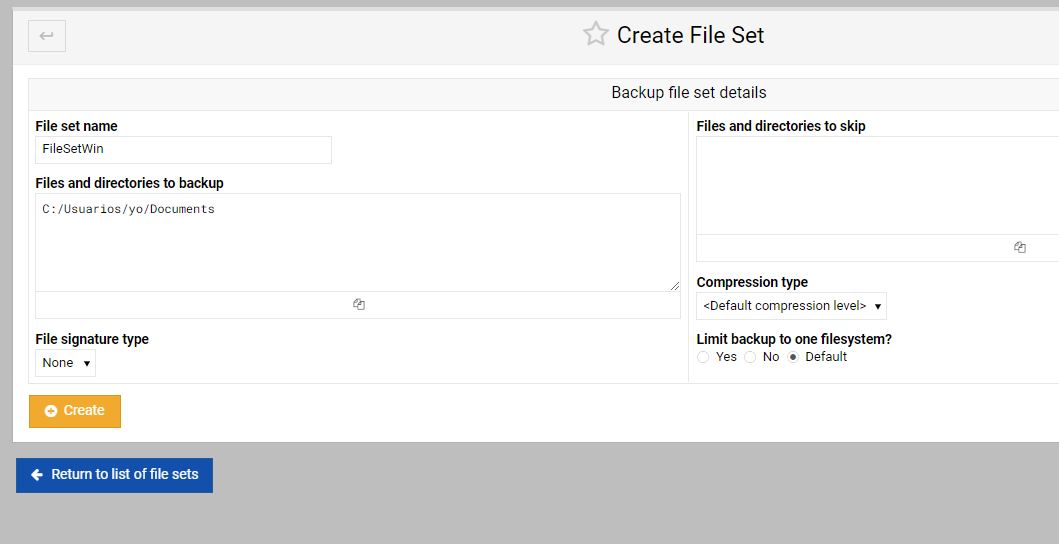
\includegraphics[width=0.5\linewidth]{instalacionBacula/filesetWindows.png}
    \caption{Configuración detallada del Fileset para Windows.}
\end{figure}

\textbf{Definición del Schedule de Backup}

Especificamos cuándo se realizará el backup utilizando un schedule preexistente o creando uno nuevo.

\begin{figure}[H]
    \centering
    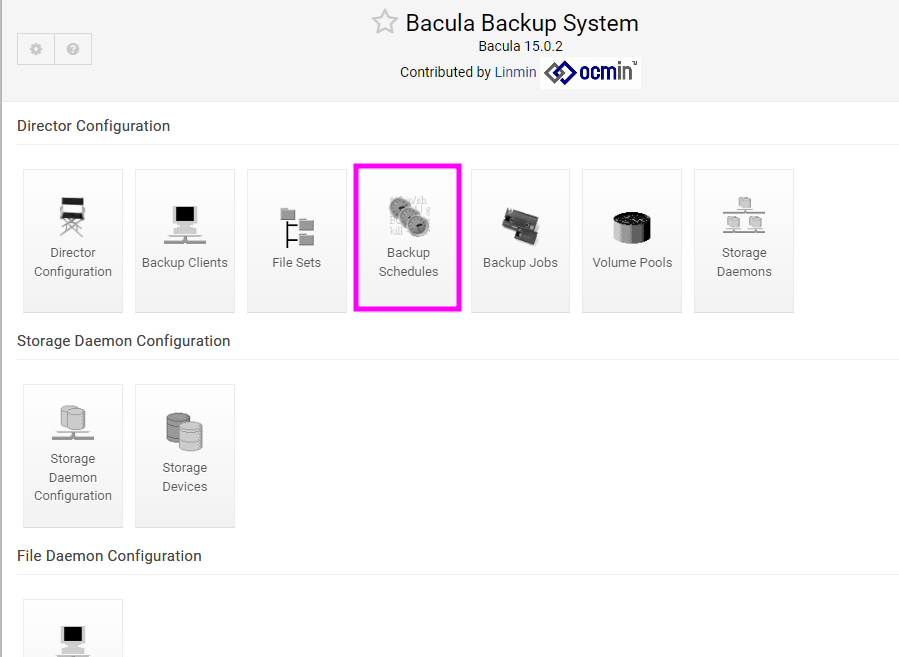
\includegraphics[width=0.5\linewidth]{instalacionBacula/schedule.png}
    \caption{Definición de un schedule de backup.}
\end{figure}

\textbf{Adición del Cliente Windows}

Procedemos a añadir el cliente Windows en la sección de Backup Clients.

\begin{figure}[H]
    \centering
    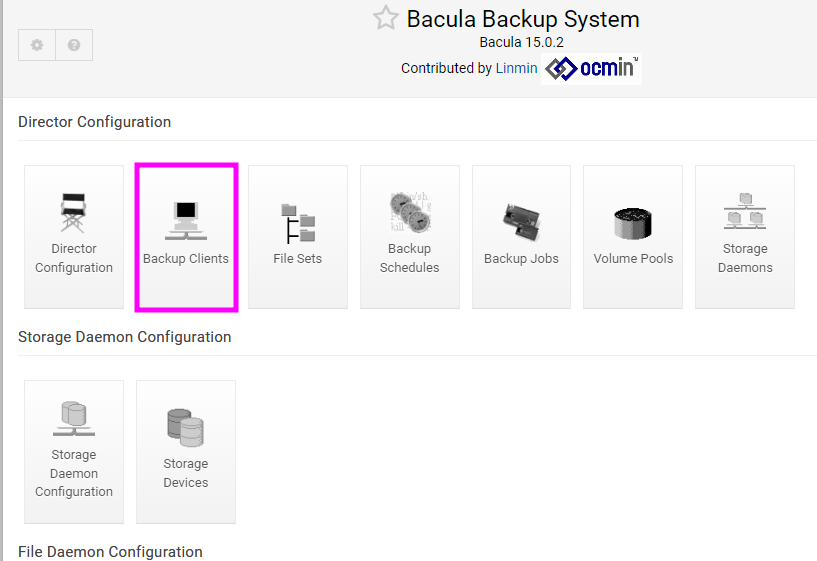
\includegraphics[width=0.5\linewidth]{instalacionBacula/asdasdas.png}
    \caption{Selección de Backup Clients.}
\end{figure}

Completamos los detalles del cliente a respaldar, incluyendo nombre, contraseña, dirección IP, y configuraciones relacionadas con TLS si es necesario.

\begin{figure}[H]
    \centering
    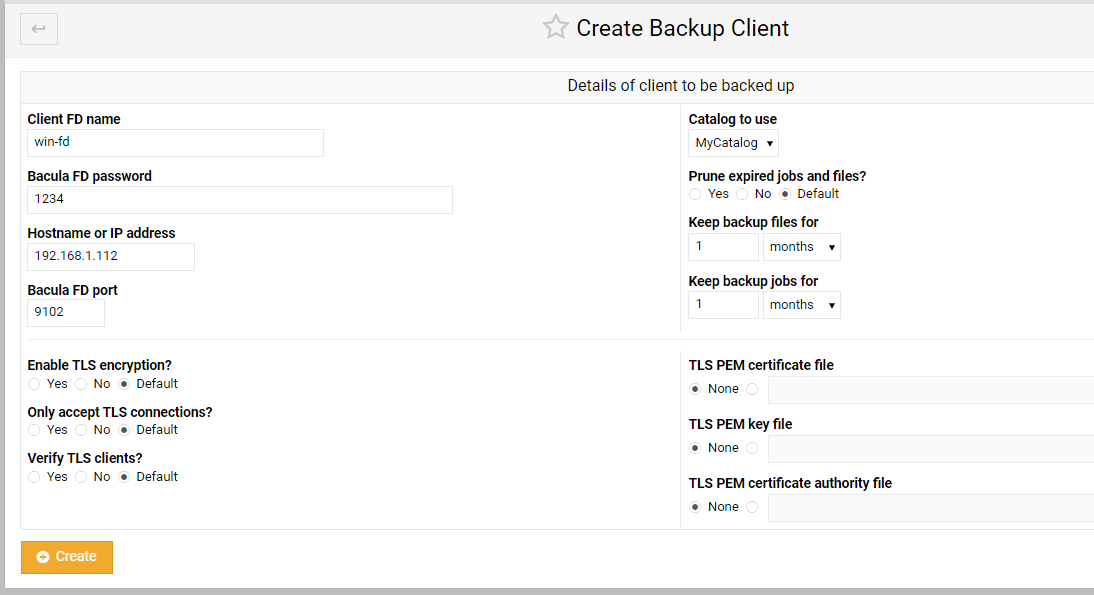
\includegraphics[width=0.5\linewidth]{instalacionBacula/createbackupclientwindows.png}
    \caption{Creación de un nuevo cliente de backup para Windows.}
\end{figure}

\textbf{Creación y Ejecución de un Job de Backup}

Creamos un job de backup especificando todos los detalles necesarios como el tipo de backup, el cliente, el fileset y el schedule.

\begin{figure}[H]
    \centering
    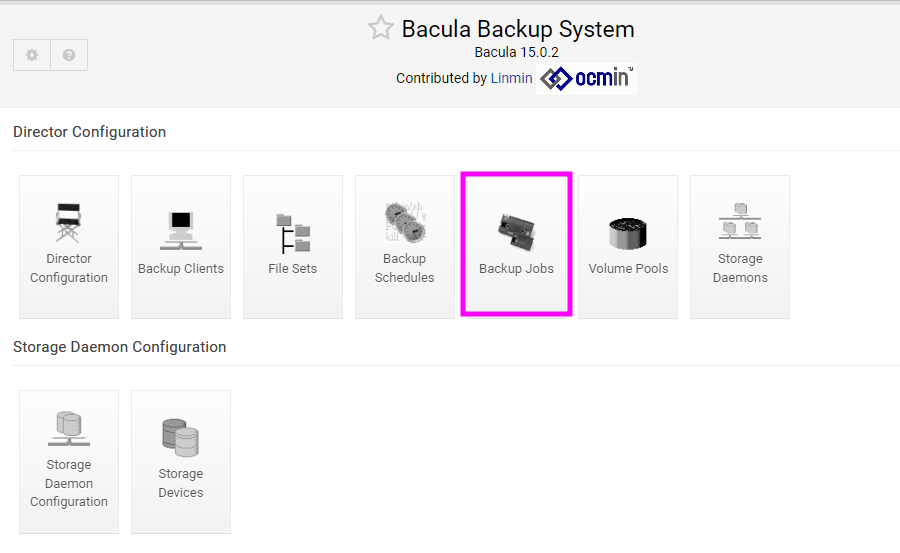
\includegraphics[width=0.5\linewidth]{instalacionBacula/createJOB.png}
    \caption{Creación de un nuevo job de backup.}
\end{figure}

Finalmente, ejecutamos el job de backup y observamos los resultados.

\begin{figure}[H]
    \centering
    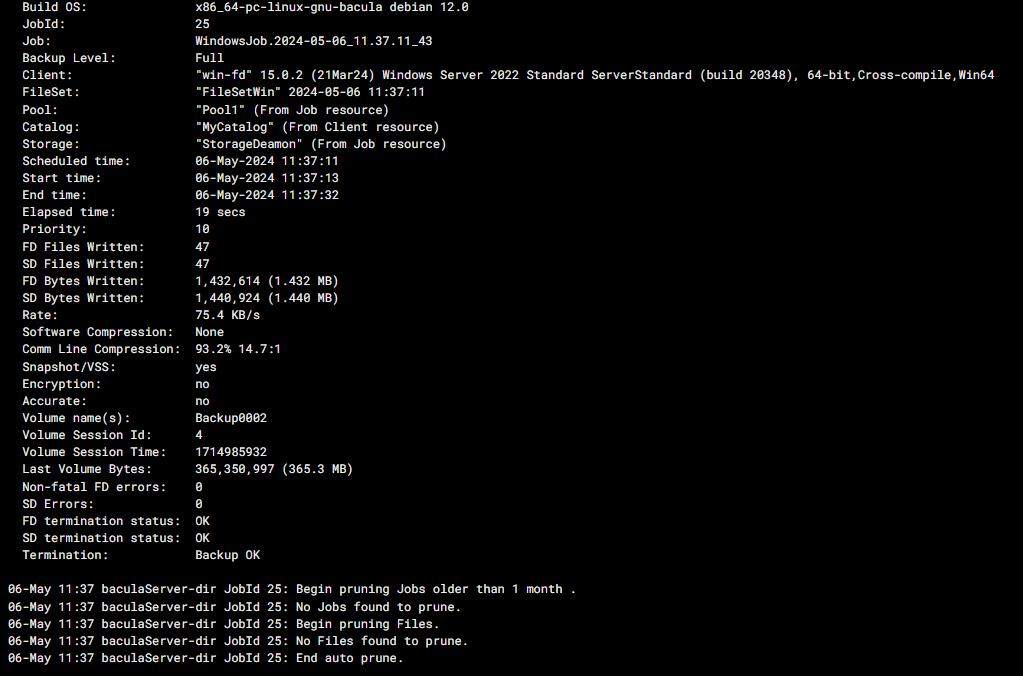
\includegraphics[width=0.5\linewidth]{instalacionBacula/backupWindows.png}
    \caption{Ejecución de un job de backup para Windows.}
\end{figure}